\documentclass[11pt,a4paper]{article}

% ============================================================================
% POLICES ET TYPOGRAPHIE
% ============================================================================
\usepackage{fontspec}
\usepackage[french]{babel}
\frenchsetup{ThinSpaceInFrenchNumbers=true}

\IfFontExistsTF{TeX Gyre Termes}{
  \setmainfont{TeX Gyre Termes}
}{
  \setmainfont{Latin Modern Roman}
}
\IfFontExistsTF{TeX Gyre Heros}{
  \setsansfont{TeX Gyre Heros}[Scale=MatchLowercase]
}{
  \setsansfont{Latin Modern Sans}[Scale=MatchLowercase]
}
\IfFontExistsTF{TeX Gyre Cursor}{
  \setmonofont{TeX Gyre Cursor}[Scale=MatchLowercase]
}{
  \setmonofont{Latin Modern Mono}[Scale=MatchLowercase]
}

% ============================================================================
% GÉOMÉTRIE ET MISE EN PAGE
% ============================================================================
\usepackage[
  a4paper,
  top=1.8cm,
  bottom=1.8cm,
  left=1.8cm,
  right=1.8cm,
  headheight=16pt
]{geometry}

\usepackage{setspace}
\setstretch{1.10}
\setlength{\parskip}{0.35em}
\setlength{\parindent}{0pt}

% ============================================================================
% COULEURS CHARTE GRAPHIQUE
% ============================================================================
\usepackage[table]{xcolor}
\definecolor{BleuInstitutionnel}{HTML}{1F3A5F}
\definecolor{BleuSecondaire}{HTML}{2E5B88}
\definecolor{GrisFonce}{HTML}{2C3E50}
\definecolor{GrisTableau}{HTML}{F8FAFC}

\usepackage{graphicx}
\usepackage{float}
\usepackage{caption}
\captionsetup{font=small,labelfont=bf,labelsep=colon}
\usepackage{booktabs}
\usepackage{tabularx}
\usepackage{array}
\usepackage{enumitem}

\newcolumntype{L}[1]{>{\raggedright\arraybackslash}p{#1}}
\newcolumntype{Y}{>{\raggedright\arraybackslash}X}

\usepackage{titlesec}
\titleformat{\section}
  {\normalfont\Large\bfseries\sffamily\color{BleuInstitutionnel}}
  {\thesection.}{0.5em}{}

\titleformat{\subsection}
  {\normalfont\large\bfseries\sffamily\color{BleuSecondaire}}
  {\thesubsection.}{0.4em}{}

\titleformat{\subsubsection}
  {\normalfont\normalsize\bfseries\sffamily\color{GrisFonce}}
  {\thesubsubsection.}{0.4em}{}

\titlespacing*{\section}{0pt}{1.4ex plus 0.3ex minus .2ex}{0.6ex plus .2ex}
\titlespacing*{\subsection}{0pt}{1.1ex plus 0.2ex minus .1ex}{0.4ex plus .1ex}

\usepackage{fancyhdr}
\pagestyle{fancy}
\fancyhf{}
\fancyhead[L]{\small\sffamily\color{BleuInstitutionnel}\bfseries Système de suivi des dépenses budgétaires}
\fancyhead[R]{\small\sffamily\color{GrisFonce} Synthèse fonctionnelle}
\fancyfoot[C]{\small\sffamily Page \thepage}
\renewcommand{\headrulewidth}{0pt}
\renewcommand{\footrulewidth}{0pt}

% Commande fluide pour les cas d'utilisation (aérée, sans cadre ni filet excessif)
\newcommand{\ficheusecase}[6]{
  \vspace{0.45em}
  {\noindent\raggedright\textbf{\sffamily\normalsize\color{BleuInstitutionnel}#1} \hfill {\scriptsize\sffamily\bfseries\color{BleuSecondaire} Acteur(s) : #2}\par}
  \vspace{0.1em}
  {\small\textbf{Finalité fonctionnelle :} #3\par}
  {\small\textbf{Conditions préalables :} #4\par}
  {\small\textbf{Déroulement des opérations :}\par
  \vspace{0.05em}
  #5\par}
  \vspace{0.05em}
  {\small\color{BleuSecondaire}\textbf{Aboutissement et variantes :} #6\par}
  \vspace{0.35em}
}

\begin{document}

% ============================================================================
% PAGE DE GARDE INSTITUTIONNELLE ÉPURÉE
% ============================================================================
\begin{titlepage}
\thispagestyle{empty}

\vspace*{2.0cm}

\begin{center}
  {\large\sffamily\bfseries\color{BleuInstitutionnel} SYSTÈME D'INFORMATION DE GESTION ADMINISTRATIVE ET FINANCIÈRE}\\[0.25cm]
  {\normalsize\sffamily\color{GrisFonce} Dématérialisation et sécurisation de la chaîne de la dépense budgétaire}

  \vspace{3.5cm}

  {\fontsize{26}{32}\selectfont\sffamily\bfseries\color{BleuInstitutionnel} Document de Synthèse}\\[0.6cm]
  {\fontsize{16}{22}\selectfont\sffamily\color{BleuSecondaire} Modélisation des Cas d'Utilisation et Spécifications Métier}\\[1.2cm]

  {\normalsize\itshape\color{GrisFonce}
    Organisation des intervenants, diagramme général unifié\\
    et fiches descriptives des services applicatifs
  }

  \vfill

  \begin{minipage}{0.85\linewidth}
    \centering\small\sffamily\color{GrisFonce}
    \textbf{Projet :} Suivi informatisé des dépenses budgétaires\\[0.15cm]
    \textbf{Livrable :} Analyse fonctionnelle et catalogue des use cases\\[0.15cm]
    \textbf{Périmètre :} De l'expression du besoin à la prise en charge au Trésor public\\[0.15cm]
    \textbf{Édition :} \today
  \end{minipage}

  \vspace{1.5cm}
\end{center}

\end{titlepage}

\newpage

% ============================================================================
% 1. INTRODUCTION ET TABLEAU SYNTHÉTIQUE
% ============================================================================
\section{Cadre opérationnel et tableau synthétique des acteurs}

L'exécution des dépenses publiques s'articule autour d'une succession d'actes administratifs, financiers et comptables régis par le principe fondamental de séparation des fonctions. L'application unifie l'\textbf{Ordonnateur} (initiative, passation et liquidation), le \textbf{Fournisseur} (soumission, livraison et facturation), le \textbf{Comptable matière} (constatation physique et attestation de service fait), le \textbf{Contrôleur financier} (régulation budgétaire préalable, réservation des crédits et visas) et le \textbf{Comptable public} (prise en charge du mandat en vue du paiement effectif).

Conformément aux directives de cadrage, l'ancienne colonne consacrée aux responsabilités juridiques abstraites a été retirée afin de focaliser la synthèse sur les attributions concrètes, les opérations applicatives et les flux d'échanges mutuels.

\vspace{0.2cm}
\begin{center}
\scriptsize
\renewcommand{\arraystretch}{1.12}
\begin{tabularx}{\linewidth}{L{2.4cm} L{3.1cm} Y L{2.7cm}}
\toprule
\textbf{\sffamily Acteur} &
\textbf{\sffamily Rôle dans le processus} &
\textbf{\sffamily Principales opérations réalisées dans le système} &
\textbf{\sffamily Autres acteurs en interaction} \\
\midrule
\rowcolor{GrisTableau}
\textbf{Ordonnateur} &
Initiateur de la commande, autorité d'engagement juridique, de liquidation et d'ordonnancement &
\begin{itemize}[leftmargin=1.0em, nosep]
  \item Exprimer et publier un besoin d'achat (UC01)
  \item Rédiger et soumettre le projet d'acte juridique au CF (UC04)
  \item Signer l'acte juridique après visa budgétaire préalable (UC05)
  \item Enregistrer et valider les factures déposées par le créancier (UC15)
  \item Arrêter le montant net exigible lors de la liquidation (UC16)
  \item Émettre, signer et transmettre le projet d'ordonnancement (UC17)
\end{itemize} &
\begin{itemize}[leftmargin=1.0em, nosep]
  \item Fournisseur
  \item Contrôleur financier
  \item Comptable matière
\end{itemize} \\
\midrule
\textbf{Fournisseur} &
Opérateur économique soumissionnaire, prestataire titulaire et créancier de l'administration &
\begin{itemize}[leftmargin=1.0em, nosep]
  \item Parcourir et consulter les expressions de besoin ouvertes (UC02)
  \item Déposer une offre technique et financière complète (UC03)
  \item Introduire une demande officielle de paiement (UC12)
  \item Téléverser factures et pièces justificatives (UC13)
  \item Suivre en temps réel l'avancement de ses dossiers de règlement (UC14)
\end{itemize} &
\begin{itemize}[leftmargin=1.0em, nosep]
  \item Ordonnateur
  \item Comptable matière
\end{itemize} \\
\midrule
\rowcolor{GrisTableau}
\textbf{Contrôleur financier} &
Garant de la discipline budgétaire, de la disponibilité des crédits et de la régularité des actes &
\begin{itemize}[leftmargin=1.0em, nosep]
  \item Réserver préventivement les crédits sur la ligne budgétaire (UC07)
  \item Accorder le quitus sur la classification en nature économique (UC08)
  \item Instruire et accorder le visa préalable sur l'acte juridique (UC06)
  \item Contrôler la régularité du projet d'ordonnancement (UC19)
  \item Signer et transmettre le dossier d'ordonnancement au Trésor (UC18)
\end{itemize} &
\begin{itemize}[leftmargin=1.0em, nosep]
  \item Ordonnateur
  \item Comptable public
\end{itemize} \\
\midrule
\textbf{Comptable matière} &
Agent assermenté garant de la réception physique, de la conformité et de l'entrée en matière &
\begin{itemize}[leftmargin=1.0em, nosep]
  \item Prendre en charge et constater contradictoirement les livraisons (UC09)
  \item Établir, valider et délivrer le procès-verbal de réception (UC10)
  \item Notifier officiellement l'ordonnateur de la conformité du service fait (UC11)
\end{itemize} &
\begin{itemize}[leftmargin=1.0em, nosep]
  \item Fournisseur
  \item Ordonnateur
\end{itemize} \\
\midrule
\rowcolor{GrisTableau}
\textbf{Comptable public} &
Autorité comptable assignataire chargée de la prise en charge des mandats d'ordonnancement &
\begin{itemize}[leftmargin=1.0em, nosep]
  \item Réceptionner et prendre en charge le dossier d'ordonnancement visé en vue du paiement effectif (UC18)
\end{itemize} &
\begin{itemize}[leftmargin=1.0em, nosep]
  \item Contrôleur financier
\end{itemize} \\
\bottomrule
\end{tabularx}
\vspace{0.15cm}
\captionof{table}{Synthèse restructurée des acteurs, attributions opérationnelles et flux d'interaction}
\label{tab:synthese_acteurs}
\end{center}

\newpage

% ============================================================================
% 2. GRAND DIAGRAMME UNIFIÉ LISIBLE EN PORTRAIT (90% DE LA PAGE)
% ============================================================================
\thispagestyle{empty}
\vspace*{-0.8cm}
\begin{center}
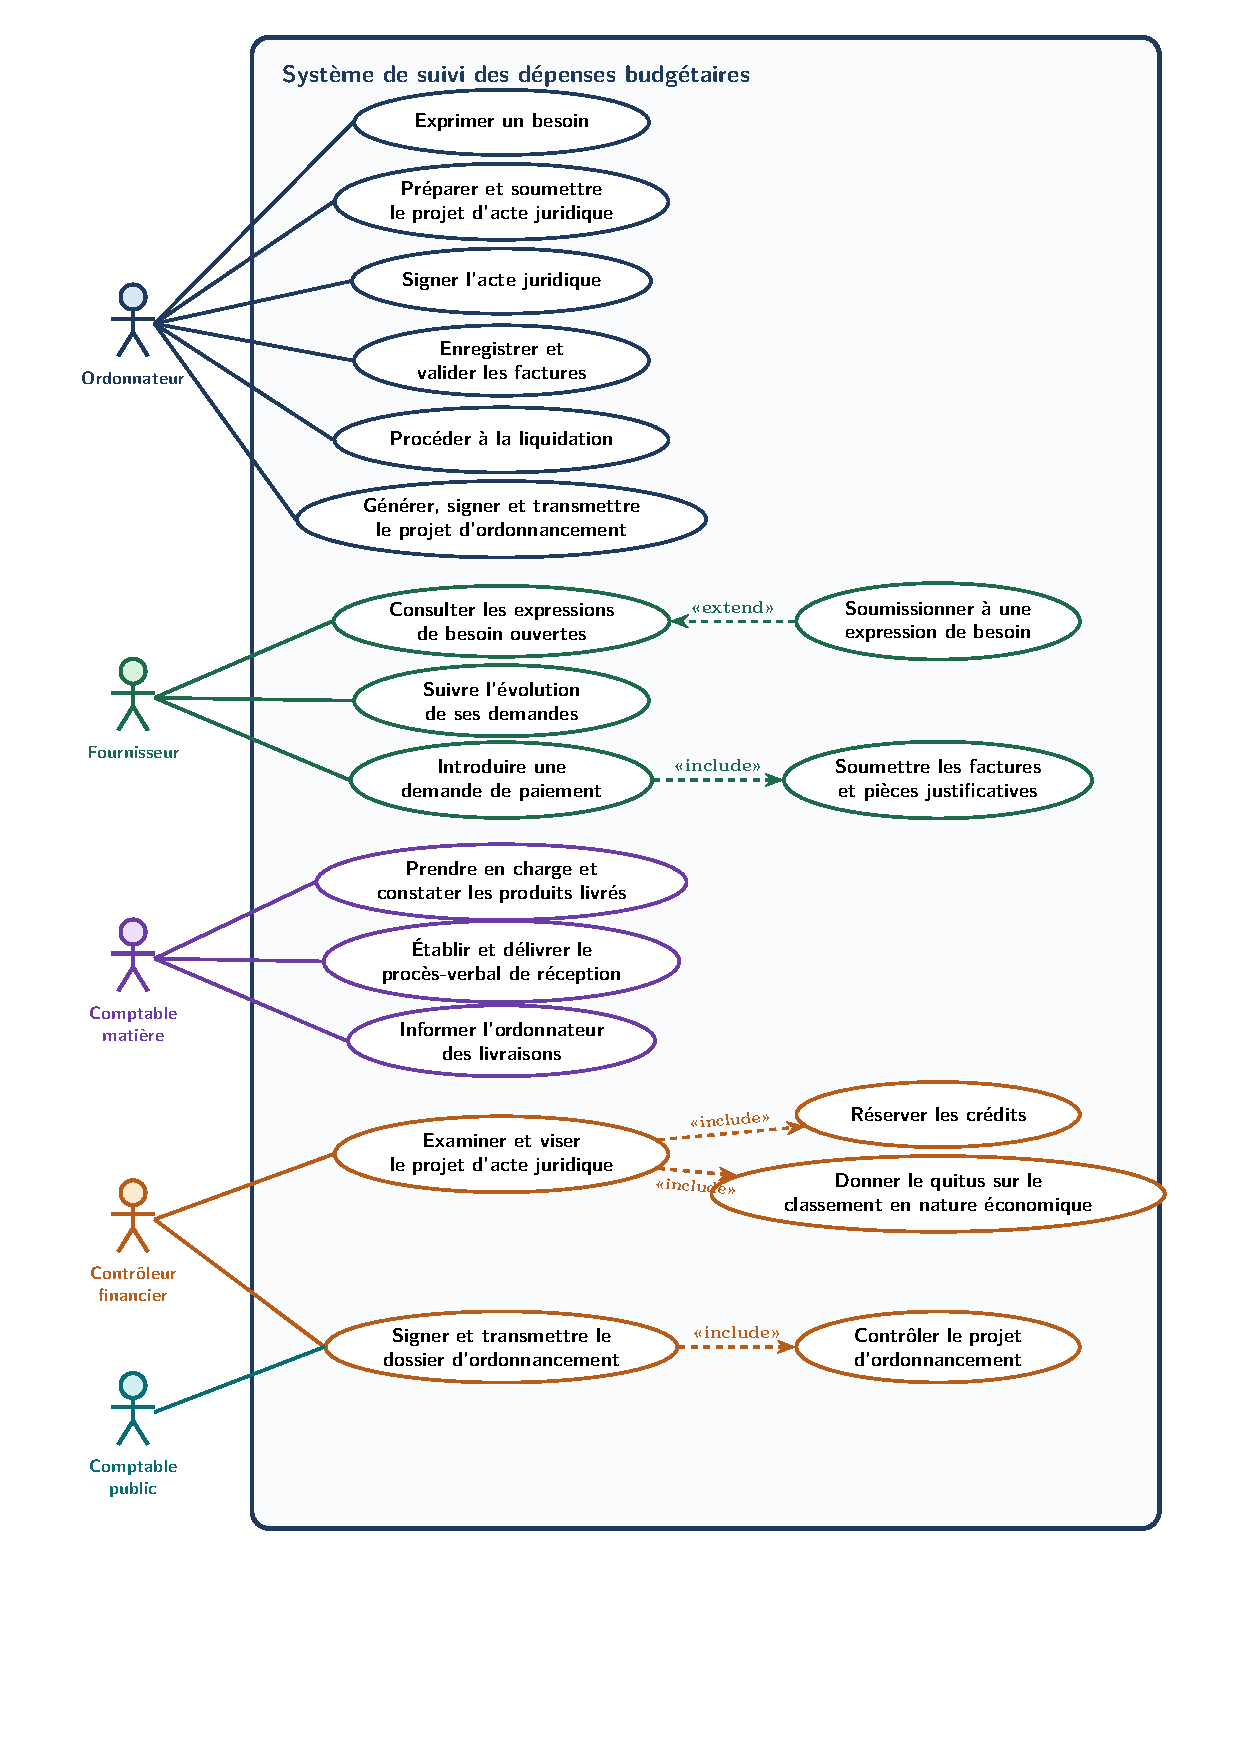
\includegraphics[width=0.98\linewidth,height=0.91\textheight,keepaspectratio]{../diagrammes/cas-utilisation-portrait.pdf}
\vspace{0.15cm}
\captionof{figure}{Diagramme général unifié des cas d'utilisation UML}
\label{fig:uc_general_unifie}
\end{center}

\newpage

% ============================================================================
% 3. DESCRIPTION TEXTUELLE DÉTAILLÉE DES CAS D'UTILISATION
% ============================================================================
\section{Description textuelle détaillée des cas d'utilisation}

La chaîne de dématérialisation de la dépense se déploie à travers quatre phases chronologiques cohérentes, couvrant l'ensemble des 19 cas d'utilisation du système.

\subsection{Phase 1 : Expression du besoin et mise en concurrence}

Cette étape initiale permet aux services gestionnaires d'extérioriser leurs besoins et d'organiser la consultation transparente des opérateurs économiques.

\ficheusecase{UC01 : Exprimer un besoin}
{Ordonnateur}
{Permettre à l'autorité gestionnaire de définir et publier un besoin d'achat de biens ou de prestations dans le système.}
{L'ordonnateur est identifié avec un compte doté des privilèges de création de dossiers d'achat.}
{1. L'ordonnateur initialise une nouvelle fiche de besoin, en renseigne la désignation, les spécifications techniques et les quantités.\par
2. Il fixe les conditions de recevabilité des offres et la date limite de soumission.\par
3. Après validation du dossier récapitulatif, il publie l'avis dans l'espace accessible aux opérateurs économiques.}
{Le besoin est publié sous le statut « Ouvert aux soumissions ». L'enregistrement préalable à l'état de brouillon modifiable reste accessible à tout moment.}

\ficheusecase{UC02 : Consulter les expressions de besoin ouvertes}
{Fournisseur}
{Offrir aux candidats potentiels la visibilité sur les consultations en cours afin d'identifier des opportunités d'affaires.}
{Le portail public des marchés de l'application est accessible sans restriction.}
{1. Le fournisseur accède au registre central des expressions de besoin actives.\par
2. Il utilise les outils de filtrage par famille de prestations, date d'échéance ou mot-clé.\par
3. Il sélectionne une consultation et télécharge l'intégralité du cahier des charges et des pièces associées.}
{Les caractéristiques complètes du besoin sont portées à la connaissance du prestataire. Ce cas d'utilisation constitue le point d'extension naturel de UC03.}

\ficheusecase{UC03 : Soumissionner à une expression de besoin (« extend » UC02)}
{Fournisseur}
{Déposer une proposition technique, financière et administrative en réponse à un besoin ouvert.}
{L'expression de besoin est en cours de validité et la date limite de remise n'est pas expirée.}
{1. À partir de la consultation d'un besoin (UC02), le fournisseur active la commande de dépôt de candidature.\par
2. Il renseigne son offre tarifaire et téléverse les justificatifs légaux, administratifs et techniques requis.\par
3. Il valide formellement sa soumission et reçoit un récépissé de dépôt électronique scellé et horodaté.}
{L'offre est enregistrée de façon inaltérable dans le système. Dès franchissement de l'échéance, tout nouveau dépôt est automatiquement verrouillé.}

\subsection{Phase 2 : Engagement juridique et contrôle budgétaire préalable}

L'engagement juridique formalise le lien contractuel entre l'organisme et le fournisseur retenu, sous la condition suspensive stricte du visa budgétaire préalable du Contrôleur financier.

\ficheusecase{UC04 : Préparer et soumettre le projet d'acte juridique}
{Ordonnateur (secondaire : Contrôleur financier)}
{Élaborer le projet de contrat ou bon de commande et le déférer à la censure budgétaire préalable.}
{Le fournisseur attributaire a été formellement retenu à l'issue de l'analyse des offres.}
{1. L'ordonnateur génère le projet d'acte juridique rattaché à l'offre retenue.\par
2. Il précise les montants convenus, le calendrier d'exécution et renseigne l'imputation budgétaire prévisionnelle.\par
3. Il télétransmet le dossier complet au Contrôleur financier pour instruction et demande de visa.}
{Le dossier passe à l'état « Soumis au contrôle budgétaire préalable », bloquant toute modification unilatérale par l'ordonnateur.}

\ficheusecase{UC06 : Examiner et viser le projet d'acte juridique (« include » UC07, UC08)}
{Contrôleur financier}
{Instruire la régularité de la dépense et accorder le visa budgétaire obligatoire autorisant la conclusion de l'engagement.}
{Un projet d'acte juridique a été régulièrement soumis par l'ordonnateur (UC04).}
{1. Le Contrôleur financier vérifie la régularité juridique des pièces et des seuils réglementaires.\par
2. Il réalise de façon indissociable la réservation des crédits budgétaires nécessaires (UC07).\par
3. Il délivre obligatoirement son quitus sur la qualification de la matière dans la nature économique (UC08).\par
4. Il appose son visa électronique favorable autorisant la formalisation de la commande.}
{L'acte est revêtu du visa budgétaire. En cas de crédits indisponibles ou d'imputation erronée, un rejet motivé renvoie le dossier à l'ordonnateur.}

\ficheusecase{UC07 : Réserver les crédits (inclus dans UC06)}
{Contrôleur financier}
{Immobiliser de manière préventive et garantie le montant prévisionnel de la dépense sur l'imputation budgétaire ciblée.}
{Instruction de l'acte juridique en cours par le Contrôleur financier.}
{1. Le système interroge le solde disponible de la ligne budgétaire désignée.\par
2. Le Contrôleur financier valide l'enveloppe nécessaire à la commande.\par
3. Les crédits correspondants sont automatiquement isolés et déduits du montant disponible.}
{Les crédits sont sanctuarisés au profit de cette dépense, prévenant tout risque de dépassement ou d'insolvabilité ultérieure.}

\ficheusecase{UC08 : Donner le quitus sur le classement en nature économique (inclus dans UC06)}
{Contrôleur financier}
{Attester de l'exacte concordance entre la nature des biens achetés et la codification économique budgétaire.}
{Instruction de l'acte juridique en cours.}
{1. Le Contrôleur financier analyse les matières et prestations désignées dans l'acte.\par
2. Il s'assure de leur parfaite conformité avec la nomenclature des comptes de dépenses.\par
3. Il formalise et enregistre son quitus de régularité d'imputation.}
{Le quitus économique est annexé au dossier, attestant du respect des règles d'affectation budgétaire.}

\ficheusecase{UC05 : Signer l'acte juridique}
{Ordonnateur}
{Apposer la signature officielle de l'administration pour conférer à la commande un caractère parfait et exécutoire.}
{Le visa favorable du Contrôleur financier a été préalablement accordé dans le système (UC06).}
{1. L'ordonnateur prend acte de la délivrance du visa budgétaire du Contrôleur financier.\par
2. Il appose sa signature d'autorité sur l'acte juridique définitif.\par
3. Le système notifie immédiatement l'acte officiel au fournisseur, l'autorisant à engager l'exécution.}
{L'acte est juridiquement exécutoire et notifié au titulaire ; le calendrier d'exécution des livraisons débute.}

\subsection{Phase 3 : Exécution des livraisons et réception matière}

Cette phase concrétise l'exécution matérielle de la commande et constate le service fait sous l'autorité du Comptable matière.

\ficheusecase{UC09 : Prendre en charge et constater les produits livrés}
{Comptable matière (secondaire : Fournisseur)}
{Accueillir physiquement les articles livrés et vérifier leur stricte conformité aux stipulations de l'acte juridique.}
{Un acte juridique valide, visé et notifié est en cours d'exécution dans l'application.}
{1. Le fournisseur présente les produits sur le site de réception avec son bordereau d'expédition.\par
2. Le Comptable matière procède à l'examen qualitatif, au décompte quantitatif contradictoire et à la vérification d'intégrité.\par
3. Il consigne l'ensemble des constatations matérielles dans le journal des réceptions du système.}
{La prise en charge physique est officialisée. En cas de non-conformité, des réserves motivées ou un refus d'admission sont enregistrés.}

\ficheusecase{UC10 : Établir et délivrer le procès-verbal de réception}
{Comptable matière (secondaire : Fournisseur)}
{Formaliser l'attestation légale de service fait et certifier l'entrée des biens dans le patrimoine administratif.}
{La constatation matérielle contradictoire s'est conclue par un avis d'admission conforme (UC09).}
{1. Le Comptable matière génère le procès-verbal de réception (PVR) récapitulant les références et quantités acceptées.\par
2. Il signe électroniquement le document d'admission.\par
3. Le procès-verbal est instantanément mis à disposition du fournisseur dans son espace personnel.}
{Le procès-verbal de réception est authentifié et scellé, constituant la preuve officielle indispensable au paiement.}

\ficheusecase{UC11 : Informer l'ordonnateur des livraisons}
{Comptable matière (secondaire : Ordonnateur)}
{Notifier l'autorité ordonnatrice de la réalisation du service fait pour lui permettre d'engager la liquidation.}
{Le procès-verbal de réception matière a été dument validé et signé (UC10).}
{1. Le Comptable matière valide la clôture des opérations de prise en charge.\par
2. Le système notifie immédiatement l'Ordonnateur et intègre les références du PV de réception sur son tableau de bord.}
{L'ordonnateur dispose de tous les éléments certifiés attestant du service fait, condition nécessaire au mandatement.}

\subsection{Phase 4 : Facturation, liquidation et ordonnancement}

La dernière phase du cycle vérifie les prétentions financières du prestataire, liquide la dette, émet l'ordre de payer et le transmet au Trésor public.

\ficheusecase{UC12 : Introduire une demande de paiement (« include » UC13)}
{Fournisseur}
{Solliciter le règlement des prestations livrées et formellement admises par le service récepteur.}
{Le fournisseur dispose d'un procès-verbal de réception matière validé dans le système (UC10).}
{1. Le fournisseur sélectionne la référence de la commande dument réceptionnée.\par
2. Il téléverse obligatoirement sa facture détaillée ainsi que ses pièces justificatives bancaires (UC13).\par
3. Il valide le dépôt de sa demande de règlement financier.}
{La demande de paiement est horodatée et transmise automatiquement au circuit d'instruction de l'Ordonnateur.}

\ficheusecase{UC13 : Soumettre les factures et pièces justificatives (inclus dans UC12)}
{Fournisseur}
{Associer à la demande de paiement l'ensemble des titres de créance certifiés et des éléments bancaires requis.}
{Demande de paiement en cours d'initialisation par le fournisseur (UC12).}
{1. Le fournisseur charge les fichiers numériques (facture normée, relevé d'identité bancaire, quittance).\par
2. Le système vérifie la conformité des formats et procède à l'horodatage et au scellement des pièces jointes.}
{Les pièces probantes de facturation sont rattachées de manière inaltérable au dossier de paiement.}

\ficheusecase{UC14 : Suivre l'évolution de ses demandes}
{Fournisseur}
{Bénéficier d'une transparence complète et en direct sur le traitement administratif de ses créances.}
{Le fournisseur est authentifié sur son portail applicatif.}
{1. Le fournisseur accède au suivi chronologique de ses demandes de paiement.\par
2. Il visualise en temps réel les étapes franchies : facture validée, dépense liquidée, mandat ordonnancé, dossier transmis au Trésor.}
{La traçabilité des délais de paiement est assurée sans nécessiter de démarches manuelles auprès des services de l'administration.}

\ficheusecase{UC15 : Enregistrer et valider les factures}
{Ordonnateur}
{Confronter la facture reçue avec le bon de commande et l'attestation de service fait pour s'assurer de sa recevabilité.}
{Une demande de paiement complète assortie de ses factures a été déposée par le fournisseur (UC12).}
{1. L'ordonnateur rapproche point par point la facture avec l'acte juridique et le procès-verbal de réception.\par
2. Il vérifie l'exactitude des calculs arithmétiques, l'application des remises et les taux de taxes.\par
3. Il prononce et enregistre la validation comptable de la facture.}
{La facture est déclarée recevable pour la liquidation. En cas d'anomalie, un rejet motivé invite le prestataire à émettre une facture rectificative.}

\ficheusecase{UC16 : Procéder à la liquidation}
{Ordonnateur}
{Arrêter et certifier avec exactitude le montant net définitif de la dette due par la collectivité au fournisseur.}
{La facture a été validée (UC15) et le service fait est dument certifié par le procès-verbal.}
{1. L'ordonnateur applique les déductions contractuelles éventuelles (pénalités pour retard de livraison, retenues de garantie, avances déjà versées).\par
2. Il arrête définitivement le montant net exigible au profit du créancier.\par
3. Il valide la mention administrative et juridique de liquidation de la dépense.}
{Le montant net de la créance est juridiquement arrêté, ouvrant droit à l'émission immédiate de l'ordre de paiement.}

\ficheusecase{UC17 : Générer, signer et transmettre le projet d'ordonnancement}
{Ordonnateur (secondaire : Contrôleur financier)}
{Émettre le mandat de paiement et soumettre le dossier complet au contrôle financier terminal.}
{La liquidation de la dépense a été formellement prononcée par l'ordonnateur (UC16).}
{1. L'ordonnateur génère le mandat d'ordonnancement reprenant les références budgétaires et le montant liquidé.\par
2. Il rassemble les pièces justificatives réglementaires (contrat visé, PVR, facture validée, décompte de liquidation).\par
3. Il appose sa signature d'autorité et transmet par voie électronique le dossier au Contrôleur financier.}
{Le projet d'ordonnancement est reçu par le Contrôleur financier pour examen réglementaire terminal.}

\ficheusecase{UC18 : Signer et transmettre le dossier d'ordonnancement (« include » UC19)}
{Contrôleur financier (secondaire : Comptable public)}
{Clore les vérifications budgétaires, signer le mandat et l'acheminer à l'agent comptable du Trésor pour paiement.}
{Le projet d'ordonnancement complet a été adressé par l'Ordonnateur (UC17).}
{1. Le Contrôleur financier exécute obligatoirement les vérifications réglementaires approfondies (UC19).\par
2. Il confirme l'imputation définitive sur la réservation de crédits opérée lors de l'engagement initial.\par
3. Il appose sa signature électronique officielle sur le mandat.\par
4. Le système transmet automatiquement le dossier complet d'ordonnancement au Comptable public.}
{Le mandat est revêtu des signatures exécutoires et mis à la disposition du Comptable public pour décaissement effectif.}

\ficheusecase{UC19 : Contrôler le projet d'ordonnancement (inclus dans UC18)}
{Contrôleur financier}
{Vérifier la complétude des justificatifs, l'exactitude de la liquidation et la parfaite cohérence de la chaîne de dépense.}
{Dossier d'ordonnancement en cours d'instruction par le Contrôleur financier.}
{1. Le Contrôleur financier contrôle la concordance rigoureuse entre l'acte initial, le PVR, la facture et le mandat.\par
2. Il vérifie l'absence de tout risque de double paiement et valide l'exactitude de l'assignation comptable du Trésor.}
{La régularité du mandatement est certifiée, autorisant la signature définitive du dossier par le Contrôleur financier.}

% ============================================================================
% 4. OBJETS IMMÉDIATS
% ============================================================================
\newpage
\section{Fiches des objets métier du domaine (au sens UML)}

Au sens de l'analyse orientée objet UML, un objet métier (ou entité du domaine) est une structure persistante dotée d'une identité propre, d'attributs de données, de relations et d'un cycle de vie gouverné par des changements d'état. Les opérations de consultation (comme la consultation des besoins ou le tableau de suivi des demandes) constituent des vues ou des requêtes d'interface et non des entités persistantes. De même, le projet d'acte juridique et l'acte juridique signé constituent un seul et même objet métier, dont l'état évolue au fil du circuit de validation.

\vspace{0.2cm}

\newcommand{\ficheobjet}[6]{
  \par\vspace{0.10cm}
  \noindent\begin{minipage}{\linewidth}
  \textbf{\sffamily\normalsize\color{BleuInstitutionnel}#1} \hfill {\footnotesize\sffamily\color{GrisFonce} Classe d'entité UML}\par
  \vspace{0.03cm}
  \textbf{Rôle métier :} #2\par
  \textbf{Attributs clés :} {\small\textsf{#3}}\par
  \textbf{Cycle de vie (états) :} #4\par
  \textbf{Relations métier :} #5\par
  \textbf{Cas d'utilisation associés :} #6\par
  \vspace{0.06cm}\hrule height 0.4pt \color{gray!25}\par
  \end{minipage}\par
}

\ficheobjet{ExpressionBesoin}
{Formalisation du besoin d'achat initial émis par le service demandeur pour autoriser la consultation.}
{idBesoin, dateEmission, objet, quantiteEstimee, montantEstime, statut}
{Brouillon $\rightarrow$ Validée $\rightarrow$ Publiée $\rightarrow$ Clôturée}
{Origine de 1..* Soumissions ; Référence pour l'ActeJuridique.}
{UC01 (Création et validation), UC02 (Consultation des besoins ouverts).}

\ficheobjet{Soumission}
{Offre technique et financière formalisée par un opérateur économique candidat.}
{idSoumission, dateDepot, montantPropose, delaiExecution, statut}
{Déposée $\rightarrow$ Recevable $\rightarrow$ Retenue / Rejetée}
{Liée à 1 ExpressionBesoin ; Peut donner lieu à 1 ActeJuridique si retenue.}
{UC03 (Enregistrement de la soumission).}

\ficheobjet{ActeJuridique}
{Contrat, marché public ou bon de commande matérialisant l'engagement juridique entre l'administration et le titulaire. Le projet d'acte et l'acte signé constituent le même objet à des stades distincts de maturité.}
{idActe, numeroContrat, montantTTC, datePreparation, dateVisa, dateSignature, statut}
{Projet $\rightarrow$ Soumis au visa $\rightarrow$ Visé CF $\rightarrow$ Signé $\rightarrow$ Notifié exécutoire}
{Issu d'une Soumission retenue ; Adossé à 1..* Crédits ; Conditionne la Facture et le PVR.}
{UC04 (Préparation du projet), UC06 (Instruction du visa), UC05 (Signature exécutoire).}

\ficheobjet{Credit}
{Dotation budgétaire disponible sur une ligne de nomenclature, faisant l'objet d'un blocage préventif pour garantir la couverture financière de la dépense.}
{idLigneCredit, imputationBudgetaire, exercice, montantAlloue, montantReserve, statut}
{Disponible $\rightarrow$ Réservé $\rightarrow$ Engagé $\rightarrow$ Soldé}
{Réservé pour 1 ActeJuridique ; Imputé définitivement sur l'Ordonnancement.}
{UC07 (Réservation préalable des crédits).}

\ficheobjet{QuitusNatureEconomique}
{Attestation formelle de conformité certifiant le classement réglementaire de la dépense dans la nomenclature économique des finances publiques.}
{idQuitus, dateQuitus, codeNomenclature, justification, statut}
{Accordé $\rightarrow$ Refusé}
{Conditionne l'octroi du Visa sur l'ActeJuridique.}
{UC08 (Contrôle et délivrance du quitus).}

\ficheobjet{Visa}
{Décision d'autorité administrative et financière délivrée par le Contrôleur financier pour valider la régularité budgétaire et juridique de l'acte.}
{idVisa, dateVisa, numeroVisa, motifEventuel, statut}
{Favorable $\rightarrow$ Favorable avec réserves $\rightarrow$ Rejeté}
{Associé à 1 ActeJuridique ou 1 Ordonnancement ; Débloque la signature exécutoire.}
{UC06 (Visa de l'acte juridique), UC18 / UC19 (Visa terminal d'ordonnancement).}

\ficheobjet{PVR (Procès-Verbal de Réception)}
{Acte authentique établi par le comptable matière attestant la livraison physique, la conformité quantitative/qualitative du service fait et la prise en charge à l'inventaire public.}
{idPVR, dateReception, lieuLivraison, conformiteTechnique, statut}
{En cours de constatation $\rightarrow$ Validé sans réserve $\rightarrow$ Validé avec réserves $\rightarrow$ Rejeté}
{Rattaché à 1 ActeJuridique ; Indispensable à la validation de la Facture et à la Liquidation.}
{UC09 (Constatation physique), UC10 (Établissement du PV), UC11 (Notification de conformité).}

\ficheobjet{DemandePaiement}
{Dossier formel de réclamation de créance déposé par le fournisseur après accomplissement des prestations.}
{idDemande, dateDepot, montantReclame, statut}
{Déposée $\rightarrow$ Recevable $\rightarrow$ En cours de traitement $\rightarrow$ Liquidée $\rightarrow$ Rejetée}
{Rassemble 1 Facture et 1..* Pièces justificatives ; Suivie en temps réel par le créancier.}
{UC12 (Introduction de la demande), UC14 (Suivi de son état d'avancement).}

\ficheobjet{Facture}
{Titre de créance financier émis par le titulaire, détaillé selon les stipulations contractuelles et contrôlé arithmétiquement par l'ordonnateur.}
{idFacture, numeroFacture, dateFacture, montantHT, montantTVA, montantTTC, statut}
{Déposée $\rightarrow$ Validée conforme $\rightarrow$ Rejetée $\rightarrow$ Rattachée à liquidation}
{Intégrée dans 1 DemandePaiement ; Rapprochée du PVR et de l'ActeJuridique.}
{UC13 (Dépôt dématérialisé), UC15 (Vérification et validation comptable).}

\ficheobjet{PieceJustificative}
{Document légal ou technique probant attestant de la régularité et de la réalité des opérations (bordereau de livraison, attestation fiscale, garantie bancaire, relevé d'identité bancaire).}
{idPiece, typePiece, intituleFichier, dateTeleversement, empreinteNumerique, statut}
{Téléversée $\rightarrow$ Contrôlée conforme $\rightarrow$ Rejetée}
{Annexée à 1 DemandePaiement, 1 ActeJuridique ou 1 Ordonnancement.}
{UC13 (Téléversement), UC15 / UC17 / UC19 (Contrôle et vérification).}

\ficheobjet{Liquidation}
{Opération arithmétique et juridique certifiée arrêtant le montant net exact de la dette due au créancier après déductions (pénalités, acomptes, retenues de garantie).}
{idLiquidation, dateLiquidation, montantBrut, deductionsPénalites, montantNetExigible, statut}
{En cours d'établissement $\rightarrow$ Certifiée exécutoire}
{S'appuie sur la Facture validée et le PVR ; Détermine le montant de l'Ordonnancement.}
{UC16 (Calcul et prononcé de la liquidation).}

\ficheobjet{Ordonnancement}
{Ordre officiel de paiement (mandat) émis par l'ordonnateur, contrôlé et visé par le contrôleur financier, transmis au comptable public pour prise en charge et règlement effectif.}
{idOrdonnancement, numeroMandat, dateEmission, montantNet, dateVisaCF, datePriseEnCharge, statut}
{Projet émis $\rightarrow$ Contrôlé régulier $\rightarrow$ Visé CF $\rightarrow$ Transmis au Trésor $\rightarrow$ Pris en charge}
{Conclut l'instruction de la dépense ; Impute définitivement les Crédits ; Transmis au Trésor.}
{UC17 (Émission du mandat), UC19 (Contrôle de conformité), UC18 (Visa CF et prise en charge Trésor).}

\vspace{0.4cm}
\begin{center}
  {\footnotesize\sffamily\color{GrisFonce} Fin du document de synthèse : Système de suivi des dépenses budgétaires}
\end{center}

\end{document}
